\documentclass[a1paper, 25pt]{tikzposter}
\usepackage[utf8]{inputenc}

\title{Environmental Stewardship and Ethics}
\author{Jason Huang}
\date{\today}
\institute{ICS4U0 @ John Fraser Secondary School}

\usepackage{blindtext}
\usepackage{comment}

\usetheme{Simple}

\begin{document}

\maketitle

\begin{columns}
  \column{0.5}
  \block{Negative Environmental Impacts} {
    \begin{tikzfigure}
      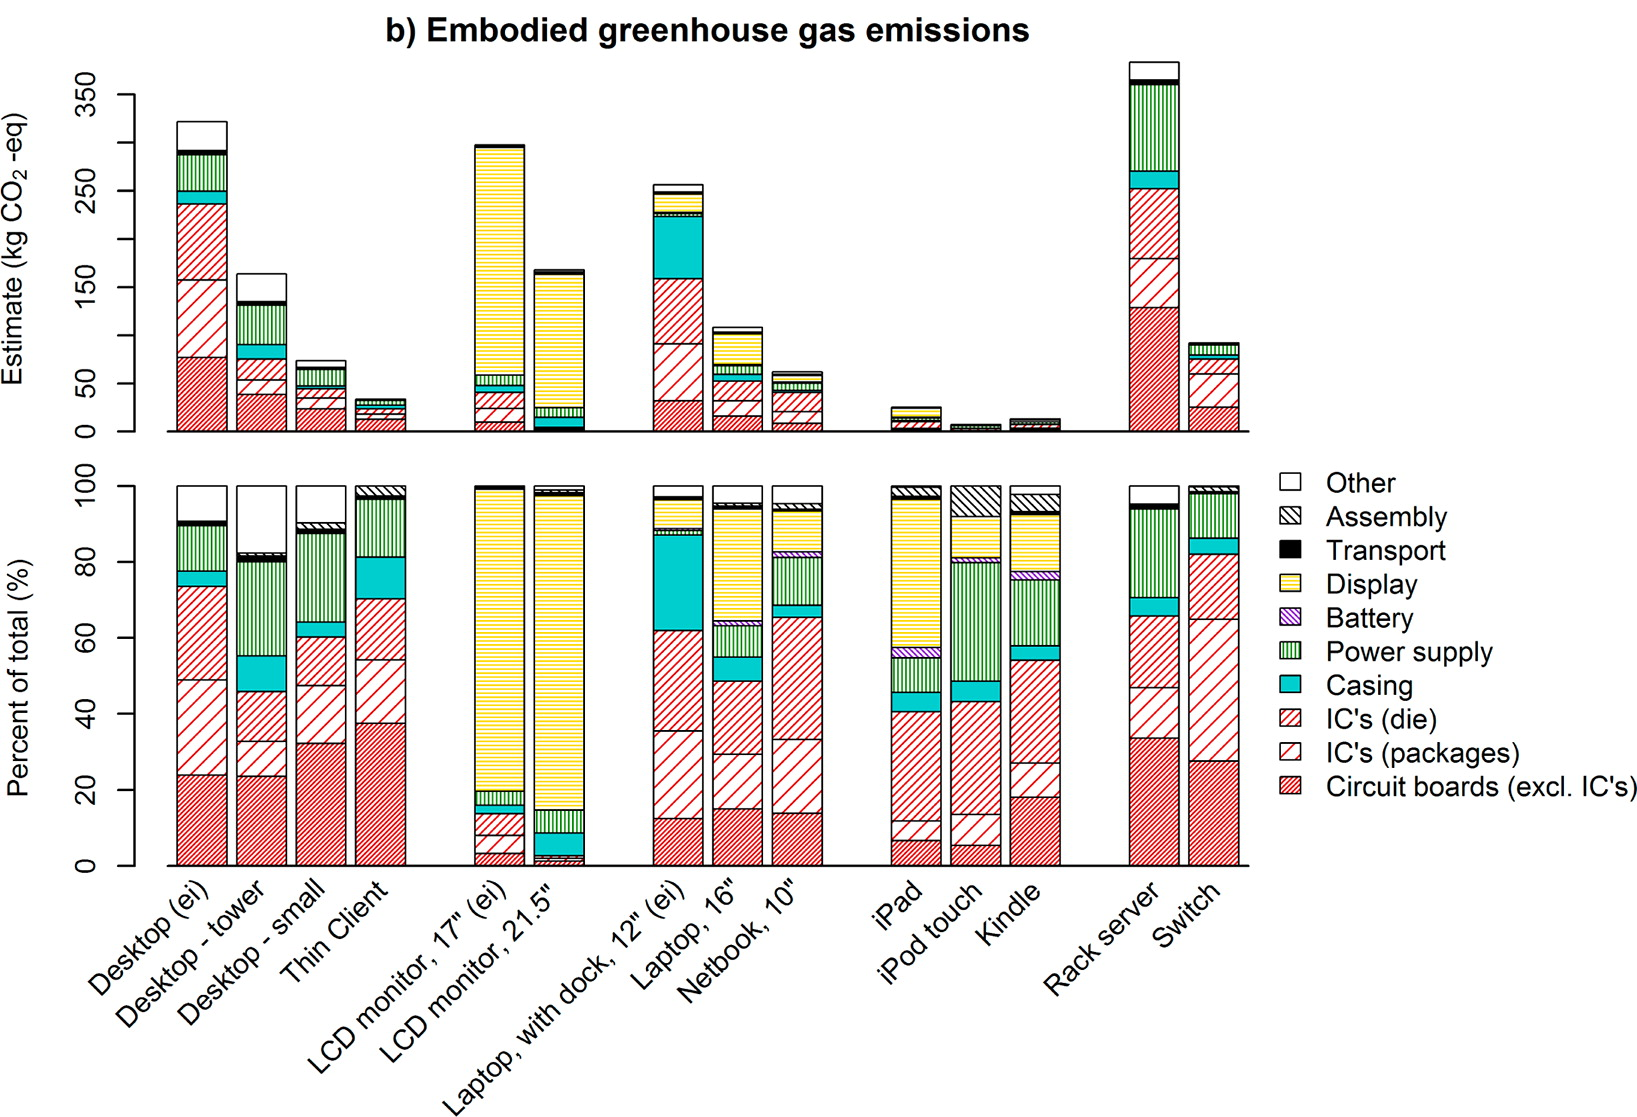
\includegraphics[width=0.4\textwidth]{images/environment.png}
    \end{tikzfigure}
    % \blindtext
    The majority of the CO2 generated from the production of devices is from display panels, which require sulfur hexafluoride for the etching of silicon. The simplest way to reduce the dependence on this chemical is to use a different process for etching involving a different chemical, such as fluorine gas, which will have a zero GWP. Some companies have already implemented full F-GHG reduction measures, but the largest players in the market, LG Display, BOE, and Samsung, have not fully implemented their proposed measures as of 2018.
  }

  \column{0.5}
  \block{Negative Health Impacts} {
    \begin{tikzfigure}
      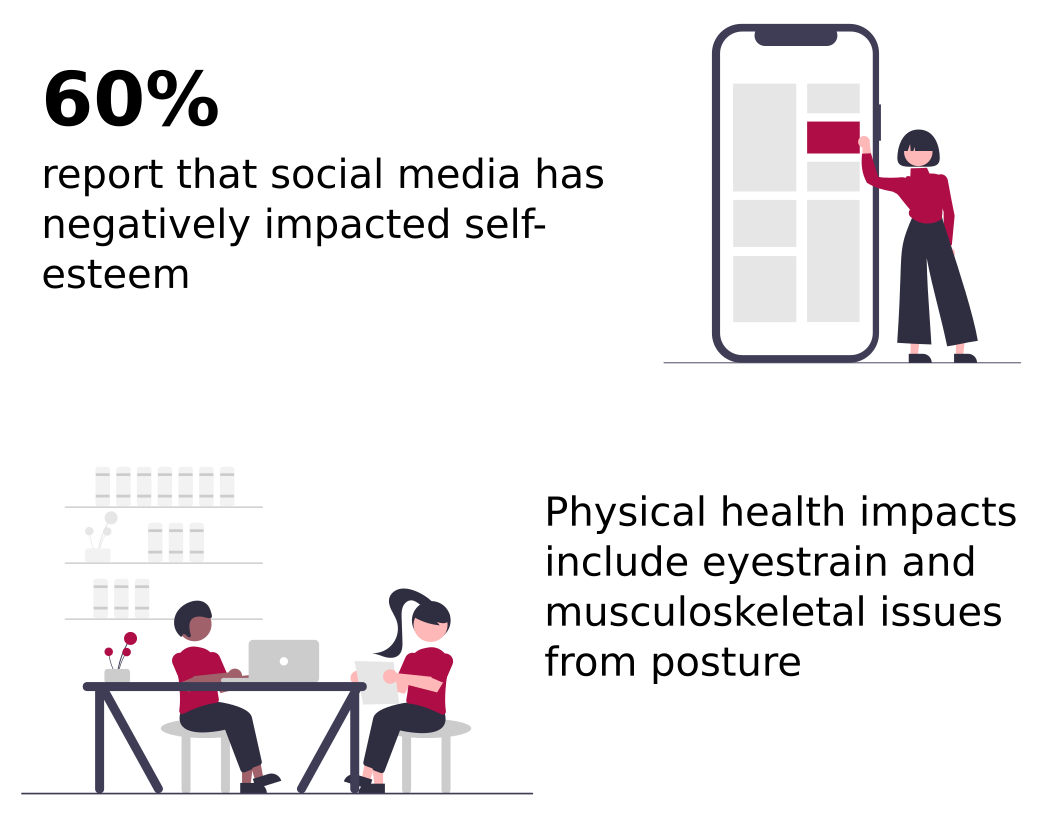
\includegraphics[width=0.4\textwidth]{images/health.png}
    \end{tikzfigure}
    Social media companies should look to reduce the toxic like-driven economy on their sites, and more resources should be given healthcare workers and services that are directly attempting to resolve the increase in mental health issues. As for physical injuries, more consumer education is required for safe computer usage to prevent RSI and back pain. Higher refresh rate displays and improvements in backlight technology may also be helpful for those who are sensitive to flickering lights, and reduce eyestrain from computer usage.
  }
\end{columns}

\begin{columns}
  \column{0.5}
  \block{Desktop Ethical Issues} {
    An ethical issue that could arise from the use of desktop computers is the continued development and use of machine learning and algorithms to replace the judgement of humans.

    For example, facial recognition and hiring/performance algorithms were mentioned in the movie \textit{Coded Bias}, with other examples being social media recommendation and filtering algorithms, such as Youtube's infamous monetization algorithm. The main problem with machine learning is that it leads to black-box algorithms that are near-impossible to understand by humans. Thus, I would propose that the use of algorithms should be monitored and regulated in certain cases. For example, hiring algorithms might be regulated by reducing the impact that they have on the hiring process, or having researchers develop a list of relatively unbiased algorithms that are permitted to be used. Understanding the thought process of an algorithm derrived from the process of machine learning is currently difficult, so funding the development of techniques to analyze such an algorithm could also be useful in determining and reducing bias.
    % \blindtext
  }
  \column{0.5}
  \block{Mobile Ethical Issues} {
    An ethical issue that could arise from the use of mobile devices is the surveillance performed by both governments and corporations.
    
    Governments commonly perform indiscriminate scraping of data, whether that be text messaging logs, public social media posts, or even chat logs from messaging services. They claim to do this to help protect the country, but surveillance agencies already have more than enough data, but are still failing to catch terrorists. The only real way to reduce this warrantless surveillance is to enforce stricter legislation against indiscriminate government surveillance, and increase organizational transparency.

    Companies also collect a lot of user data, but they use this for targeted advertising. Many social media sites have no real way to opt out of this collection, and some, such as Facebook, even collect data about users who are not signed up. The best way to give citizens more control of their data would also be to create legislation that protects customers, such as California's privacy laws or GDPR.
    % \blindtext
  }
\end{columns}

\end{document}
